\documentclass[aspectratio=169]{beamer}
%\documentclass[handout,aspectratio=169]{beamer}	%handout

\title[Harmonic Oscillator]{Harmonic Oscillator with Path Integral Monte-Carlo on the Lattice}
\author{Benedikt Otto}
\date{\printdate{31.03.2020}}
\institute{physics760: Computational Physics}

%\usetheme{Antibes}
%\usetheme{Berlin}
%\usetheme{Bergen}
%\usetheme{Boadilla}
\usetheme{Berkeley}	% gut
%\usetheme{Goettingen}
%\usetheme{Hannover}
%\usetheme{Marburg}
%\usetheme{Hannover}
%\usetheme{Hannover}
%\usecolortheme{beetle}
%\usecolortheme{dolphin}
%\usecolortheme{seahorse}
%\usecolortheme{sidebartab}
%\usecolortheme{whale}


\makeatletter
\beamer@headheight=1.5\baselineskip
\makeatother		% schmalere Titelzeile

\setbeamertemplate{footline} 
{ 
	\leavevmode% 
	\hbox{% 
		\begin{beamercolorbox}[wd=.25\paperwidth,ht=2.25ex,dp=1ex,center]{author in head/foot}% 
			\usebeamerfont{author in head/foot}Benedikt Otto%\insertshortauthor%~~(\insertshortinstitute) 
		\end{beamercolorbox}% 
		\begin{beamercolorbox}[wd=.5\paperwidth,ht=2.25ex,dp=1ex,center]{title in head/foot}% 
			\usebeamerfont{title in head/foot}\insertshorttitle
		\end{beamercolorbox}% 
		\begin{beamercolorbox}[wd=.15\paperwidth,ht=2.25ex,dp=1ex,center]{date in head/foot}% 
			\usebeamerfont{date in head/foot}\insertshortdate{}			
		\end{beamercolorbox}% 
		\begin{beamercolorbox}[wd=.1\paperwidth,ht=2.25ex,dp=1ex,right]{date in head/foot}% 
			\usebeamerfont{date in head/foot}
			\insertframenumber{}\hspace*{2ex} % / \inserttotalframenumber\hspace*{2ex} %\hspace*{2ex} 
		\end{beamercolorbox}}% 
	\vskip0pt% 
}

\newcommand{\appendixstyle}{
	\setbeamertemplate{footline} 
	{ 
		\leavevmode% 
		\hbox{% 
			\begin{beamercolorbox}[wd=.25\paperwidth,ht=2.25ex,dp=1ex,center]{author in head/foot}% 
				\usebeamerfont{author in head/foot}Benedikt Otto%\insertshortauthor%~~(\insertshortinstitute) 
			\end{beamercolorbox}% 
			\begin{beamercolorbox}[wd=.5\paperwidth,ht=2.25ex,dp=1ex,center]{title in head/foot}% 
				\usebeamerfont{title in head/foot}\insertshorttitle
			\end{beamercolorbox}% 
			\begin{beamercolorbox}[wd=.15\paperwidth,ht=2.25ex,dp=1ex,center]{date in head/foot}% 
				\usebeamerfont{date in head/foot}\insertshortdate{}			
			\end{beamercolorbox}% 
			\begin{beamercolorbox}[wd=.1\paperwidth,ht=2.25ex,dp=1ex,right]{date in head/foot}% 
				\usebeamerfont{date in head/foot}
				\insertframenumber{}*\hspace*{2ex} %\hspace*{2ex} 
		\end{beamercolorbox}}% 
		\vskip0pt% 
	}
}


%\lstnewenvironment{TeXlstlisting}{\lstset{language=[LaTeX]TeX}}{}
\usepackage{appendixnumberbeamer}
\usepackage{showexpl}
\usepackage{xcolor}
\usepackage{capt-of}
\usepackage{lipsum}
\usepackage{units}


\usepackage{listings}

%\usepackage[square,sort,comma,numbers]{natbib}
%\setbeamertemplate{bibliography item}{}
%\let\oldbibliography\thebibliography
%\renewcommand{\thebibliography}[1]{\vspace{-15px}\oldbibliography{#1}
%	\setlength{\itemsep}{-12pt}} %Reducing spacing in the bibliography.

%\setlength{\bibsep}{0pt}

%\usepackage{beamerthemesplit}

%\setcounter{tocdepth}{1}
%\setcounter{tocdepth}
\usepackage[british,UKenglish,USenglish,english]{babel}
\usepackage[utf8]{inputenc}
\usepackage{amsmath}
\usepackage{amsfonts}
\usepackage{amssymb}
\usepackage{epstopdf}
\usepackage[british]{isodate}
\usepackage{graphicx}
\usepackage{float}
\usepackage{caption}
\usepackage{graphicx}
\usepackage{subcaption}
\usepackage{geometry}
\usepackage{units}
\usepackage{amsmath}
\usepackage{csquotes}
\usepackage{tikz}
\usepackage{circuitikz}
\usepackage{listings}
\usepackage{paralist}
[decimalsymbol=comma]
\usepackage{siunitx}
\usepackage{color}
\definecolor{pink}{rgb}{1,0.5,0.5}
\makeatletter
%\renewcommand\paragraph{\@startsection{paragraph}{4}{\z@}%
%	{-2.5ex\@plus -1ex \@minus -.25ex}%
%	{1.25ex \@plus .25ex}%
%	{\normalfont\normalsize\bfseries}}
\makeatother
\setcounter{secnumdepth}{4} % how many sectioning levels to assign numbers to
\setcounter{tocdepth}{4}    % how many sectioning levels to show in ToC

\setbeamertemplate{itemize subitem}{$\bullet$}	% change subitem symbols

\beamertemplatenavigationsymbolsempty	%remove navigation symbols

\usepackage{hyperref}
\usetikzlibrary{decorations.pathmorphing}

%Define tikz bindings
\usepackage{tikz}
\usetikzlibrary{decorations.pathreplacing}
\usetikzlibrary{decorations.pathmorphing}
\usetikzlibrary{decorations.markings}
\usetikzlibrary{positioning, shapes, snakes, arrows}
\usepackage{scrextend}
\changefontsizes{13pt}		% groessere Schrift


%\tabrowsep10mm
\renewcommand{\arraystretch}{1.3}
\graphicspath{{Imgs/}}

% Titelseite
\begin{document}
\begin{frame}
	\titlepage
\end{frame}


\section{Motivation}
\begin{frame}
	\frametitle{Introduction}
	\begin{itemize}
		\item \textbf{Path integral method} method is the quantum mechanical generalisation of the \textbf{Principle of stationary Action}.
		\item Harmonic oscillator is well-understood
		\item Anharmonic oscillator serves as a toy model for the tunnelling effect
		\item Path-integral formalism used in more interesting systems as the QCD.
	\end{itemize}
\end{frame}

\section{Theory}
\begin{frame}
	\frametitle{Theory}
	\begin{itemize}
		\item Transition probability is $K(a, b) = \int_a^b e^{iS/\hbar} \mathcal Dx(t)$
		\item $\mathcal Dx(t)$ means integration over all paths starting at $a$ and resulting in $b$.
		\begin{itemize}
			\item Fast oscillations of the phase
			\item Infinite dimensional integral over infinite boundaries
			\\ $\Rightarrow$ analytically generally not solvable
		\end{itemize}
		\item transition into \textbf{Euclidean} time $t \rightarrow it$, called \textbf{Wick}-rotation
	\end{itemize}
\end{frame}

\begin{frame}
	\frametitle{Theory}
	\begin{itemize}
		\item $S = \tau \sum_i {V(x_i) + T(x_i, x_{i+1})}$
		\item only $\Delta S$ is important $\Rightarrow$ complete recalculation is not necessary
		\item $\Delta S = \tau (V(x_{i;new}) - V(x_{i;old}) + $\\$ + T(x_{i-1}, x_{i;new}) + T(x_{i;new}, x_{i+1}) - T(x_{i-1}, x_{i;old}) - T(x_{i;old}, x_{i+1}))$
		\item Potential energy: $V(x) = \mu x^2 + \lambda x^4$
		\item Kinetic energy: $T(x_1, x_2) = \frac m2 \frac{(x_1 - x_2)^2}{\tau^2}$
	\end{itemize}
\end{frame}

\section{Methods}
\begin{frame}
	\frametitle{Methods}
	\begin{itemize}
		\item Metropolis-Hastings algorithm
		\item Initialisation of the (time) lattice with for example gaussian distributed random values
		\item Iterate repeatedly over all lattice sites
		\item Draw a new value for current lattice site
		\item Evaluate $\Delta S < 0$ $\Rightarrow$ accept change
		\item Else: Accept if $e^{-\Delta S / \hbar} > x$ for $x \in [0, 1]$ evenly distributed
	\end{itemize}
\end{frame}


\section{Implementation}
\begin{frame}
	\frametitle{Implementation}
	\begin{itemize}
		\item Implemented in Python3
		\item Main loop implemented in C++ to improve performance drastically
		\item Plotting done in Python3
	\end{itemize}
\end{frame}


\section{Results}
\begin{frame}
	\frametitle{Verification: Harmonic oscillator}
	\vspace{-15px}
	\begin{columns}
		\begin{column}{0.49\textwidth}
			\begin{figure}[H]
				\centering
				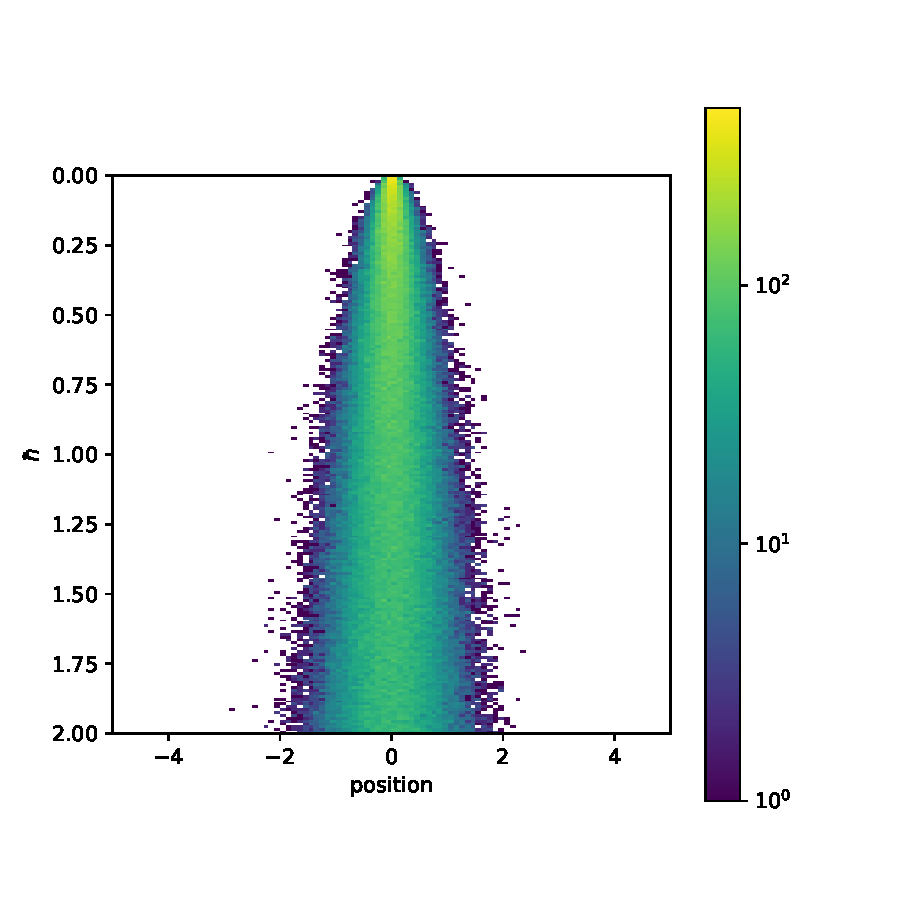
\includegraphics[width=\textwidth]{../imgs/harmonic_oscillator_classical_limit/harmonic_oscillator_10_classical_limit.pdf}
				\caption{Classical limit harmonic oscillator.}
				\label{fig:harmonic_oscillator_classical_limit}
			\end{figure}
		\end{column}
		\begin{column}{0.49\textwidth}
			\begin{itemize}
				\item Condenses into classical minimum for $\hbar \rightarrow 0$
			\end{itemize}
		\end{column}
	\end{columns}
\end{frame}


\begin{frame}
	\frametitle{Verification: Anharmonic oscillator}
	\vspace{-15px}
	\begin{columns}
		\begin{column}{0.49\textwidth}
			\begin{figure}[H]
				\centering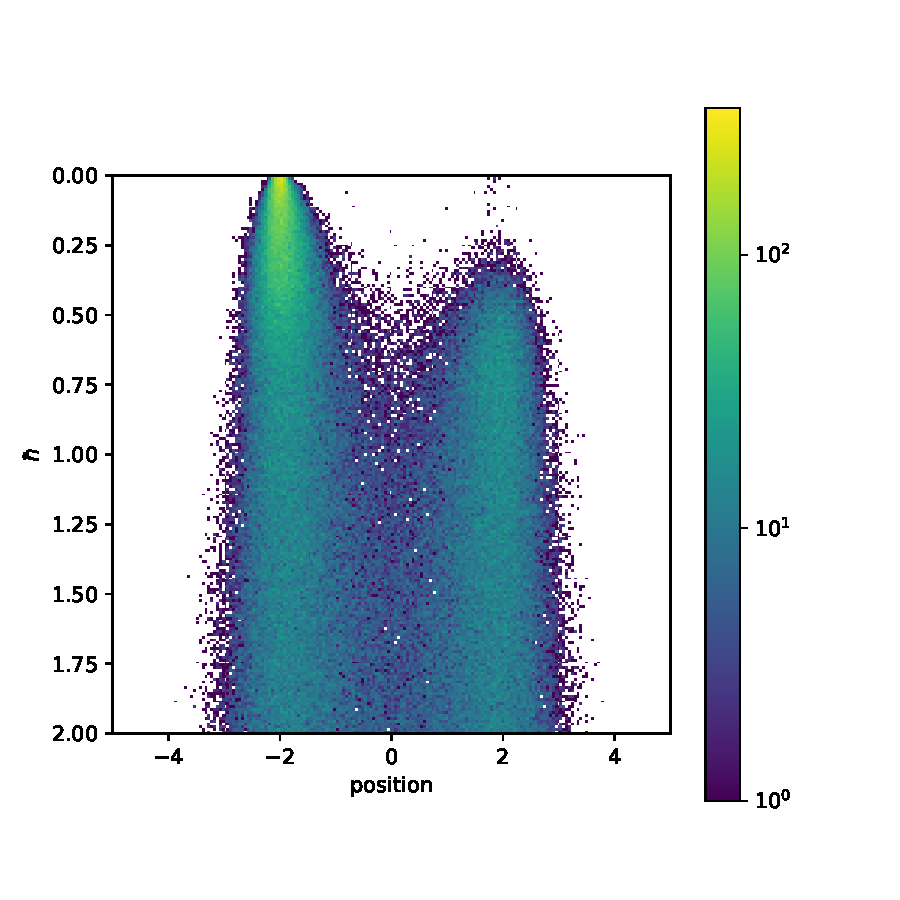
\includegraphics[width=\textwidth]{../imgs/anharmonic_oscillator_classical_limit/anharmonic_oscillator_classical_limit.pdf}
			\caption{Classical limit anharmonic oscillator.}
			\label{fig:anharmonic_oscillator_classical_limit}
			\end{figure}
		\end{column}
		\begin{column}{0.49\textwidth}
			\begin{itemize}
				\item Initially prepared in the left minimum
				\item Condenses into classical minimum for $\hbar \rightarrow 0$
				\item For low $\hbar$ right minimum is not populated
			\end{itemize}
		\end{column}
	\end{columns}
\end{frame}


\begin{frame}
	\frametitle{Verification: Gaussian shape}
	\vspace{-15px}
	\begin{columns}
		\begin{column}{0.6\textwidth}
			\begin{figure}[H]
				\centering
					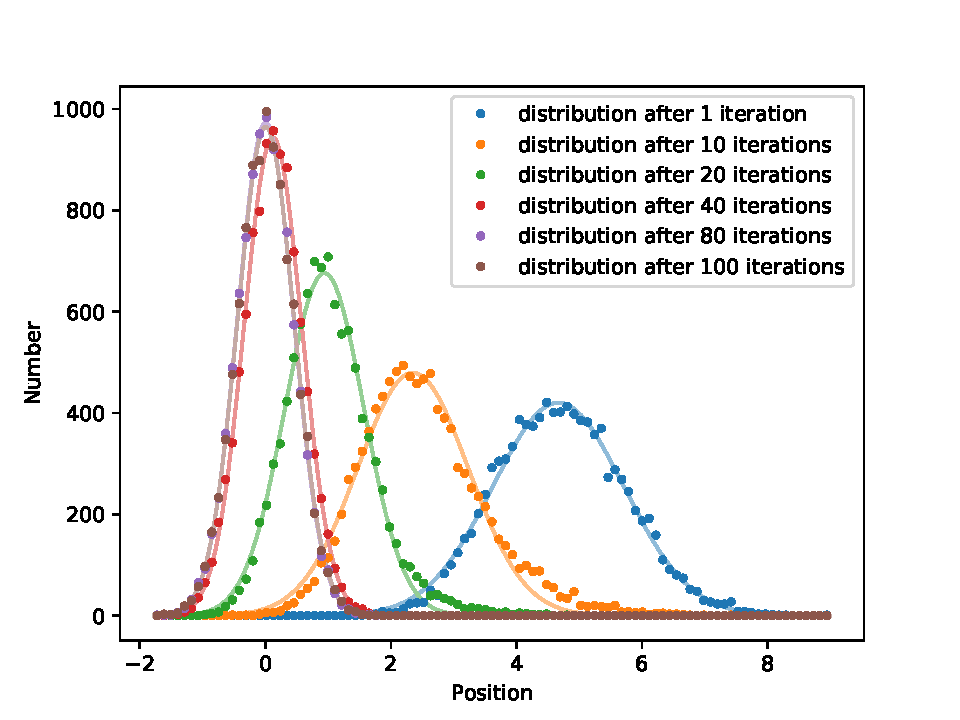
\includegraphics[width=\textwidth]{../imgs/harmonic_oscillator_track/track_10010000_gauss_1_fit.pdf}
				\caption{Probability density with gaussian fits.}
				\label{fig:harmonic_oscillator_track_10010000_gauss_1_fit}
			\end{figure}
		\end{column}
		\begin{column}{0.39\textwidth}
			\begin{itemize}
				\item Starting with a gaussian initial distribution
				\item Strong deviation from the gaussian shape after 20 iterations
				\item Thermalisation: resume to gaussian shape after 100 iterations
			\end{itemize}
		\end{column}
	\end{columns}
\end{frame}


\begin{frame}
	\frametitle{Verification: Gaussian shape}
	\vspace{-15px}
	\begin{columns}
		\begin{column}{0.6\textwidth}
			\begin{figure}[H]
				\centering
				\begin{subfigure}[c]{0.49\textwidth}
					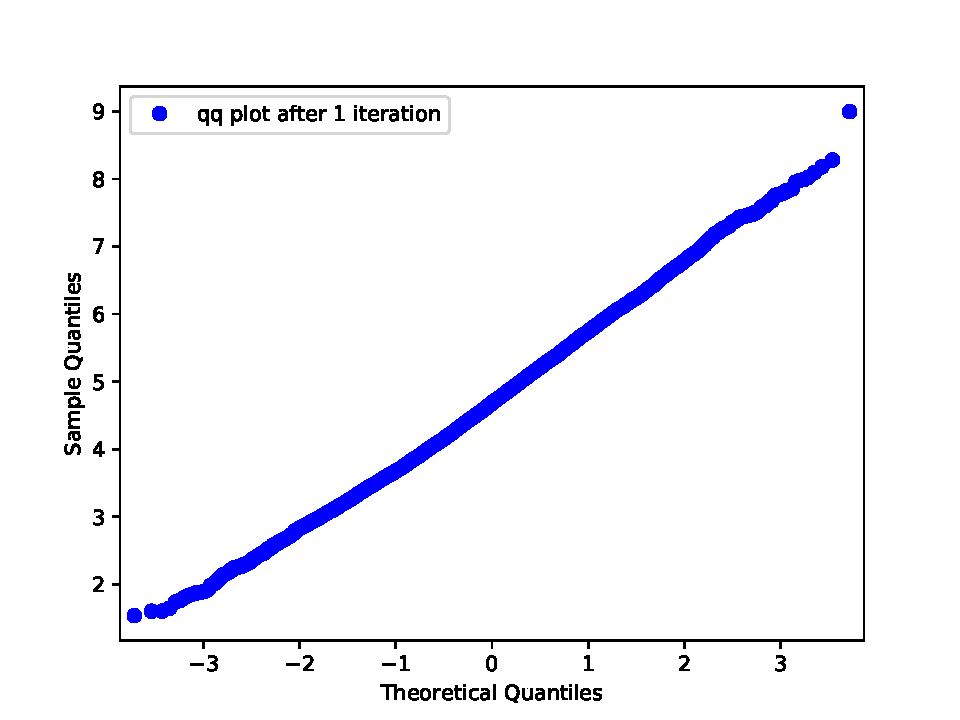
\includegraphics[width=\textwidth]{../imgs/harmonic_oscillator_track/track_10010000_qq_1.pdf}
				\end{subfigure}
				\begin{subfigure}[c]{0.49\textwidth}
					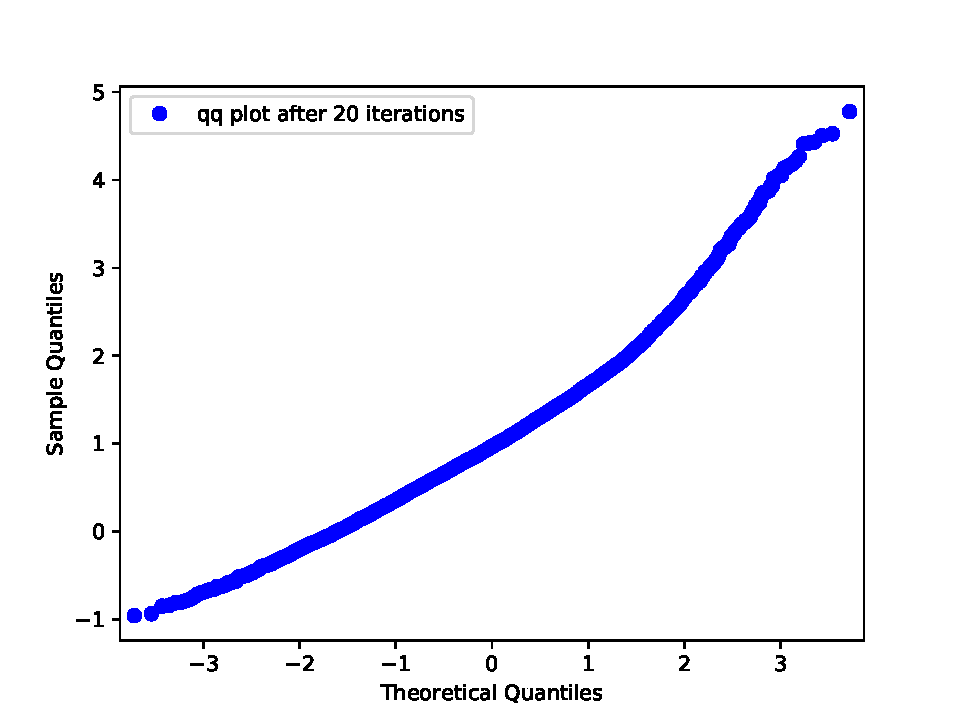
\includegraphics[width=\textwidth]{../imgs/harmonic_oscillator_track/track_10010000_qq_20.pdf}
				\end{subfigure}
				\begin{subfigure}[c]{0.49\textwidth}
					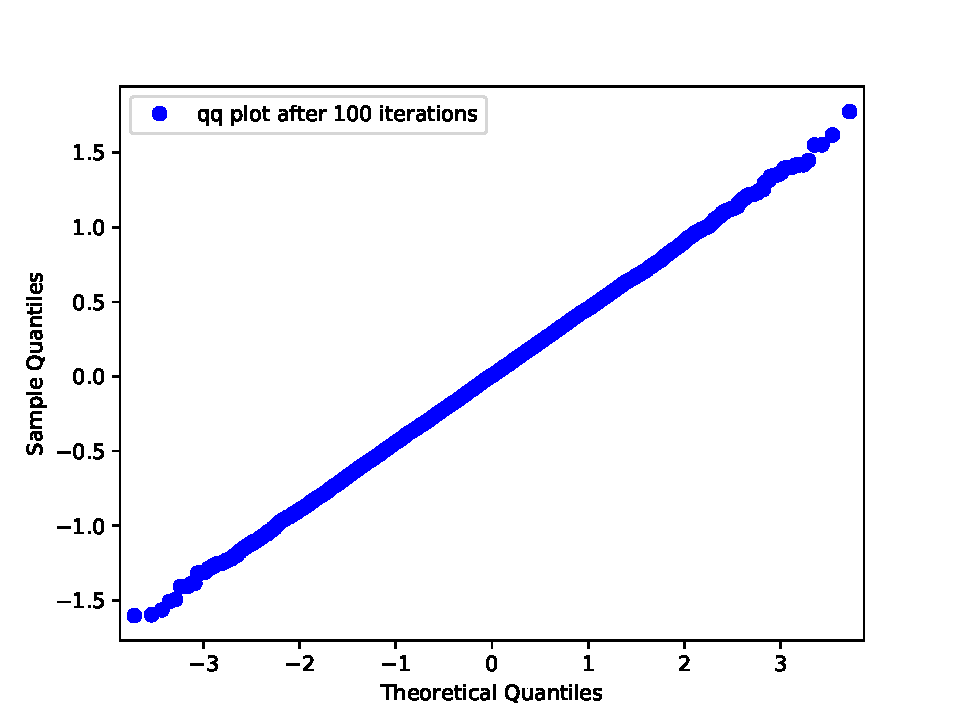
\includegraphics[width=\textwidth]{../imgs/harmonic_oscillator_track/track_10010000_qq_100.pdf}
				\end{subfigure}
				\caption{qq-plots: distribution after 1, 20 and 100 Metropolis iterations, compared with gaussian.}
				\label{fig:harmonic_oscillator_track_track_10010000_qqs}
			\end{figure}
		\end{column}
		\begin{column}{0.39\textwidth}
			\begin{itemize}
				\item Starting with a gaussian initial distribution
				\item Strong deviation from the gaussian shape after 20 iterations
				\item Thermalisation: resume to gaussian shape after 100 iterations
			\end{itemize}
		\end{column}
	\end{columns}
\end{frame}


\begin{frame}
\frametitle{}
\begin{center}
	Verification: Results match the expectation
	\\
	$\Rightarrow$ Code seems to be valid
\end{center}
\end{frame}


\begin{frame}
	\frametitle{Harmonic oscillator: Tracks}
	\vspace{-15px}
	\begin{figure}[H]
		\centering
			\begin{subfigure}[c]{0.49\textwidth}
				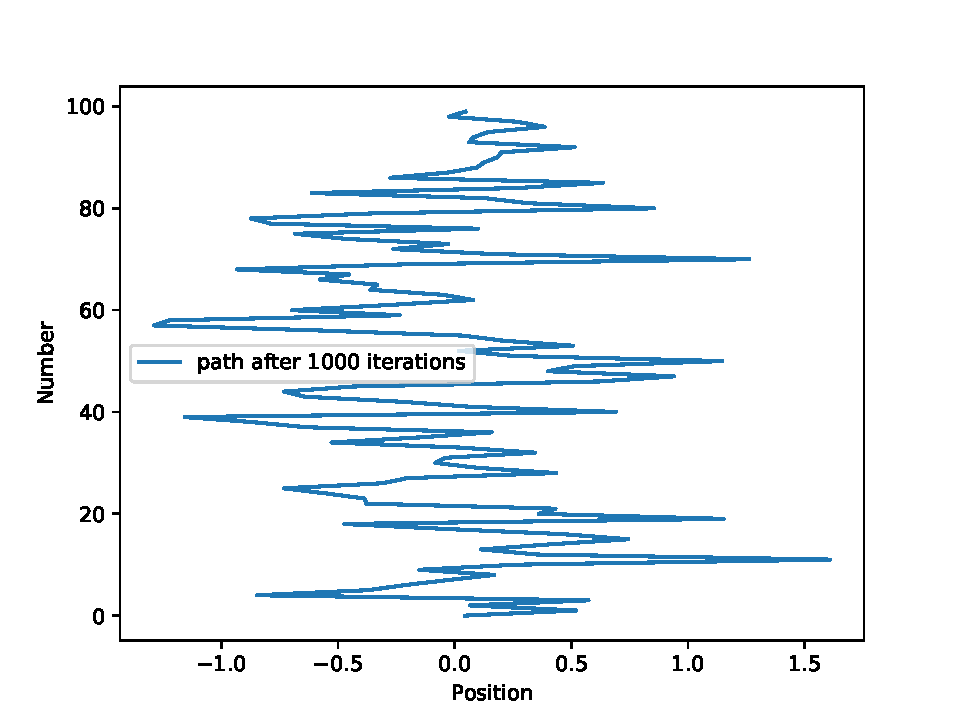
\includegraphics[width=\textwidth]{../imgs/harmonic_oscillator_track/track_1000100_track_1000.pdf}
				\caption{$m=0.25$}
				\label{fig:harmonic_oscillator_track_1000100_track_1000_light}
			\end{subfigure}
			\begin{subfigure}[c]{0.49\textwidth}
				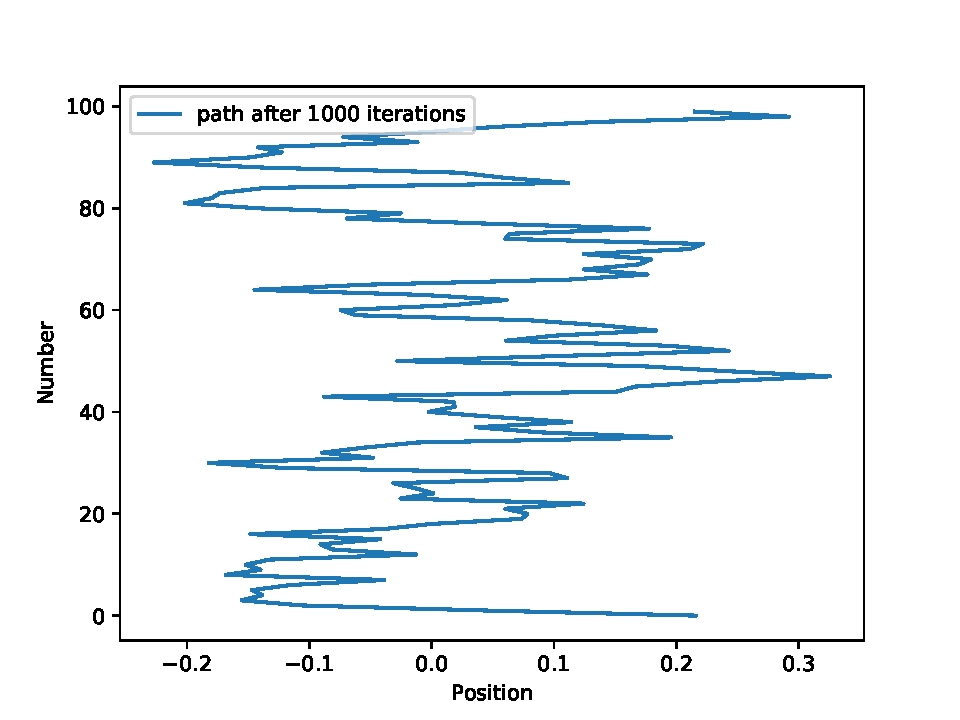
\includegraphics[width=\textwidth]{../imgs/harmonic_oscillator_track/track_1000100_heavy_track_1000.pdf}
				\caption{$m=10.0$}
				\label{fig:harmonic_oscillator_track_1000100_track_1000_heavy}
			\end{subfigure}
		\caption{Typical tracks of the harmonic oscillator.}
		\label{fig:harmonic_oscillator_track_1000100_track_1000}
	\end{figure}
\end{frame}


\begin{frame}
	\frametitle{Harmonic oscillator: Tracks}
	\vspace{-15px}
	\begin{columns}
		\begin{column}{0.6\textwidth}
			\begin{figure}[H]
				\centering
					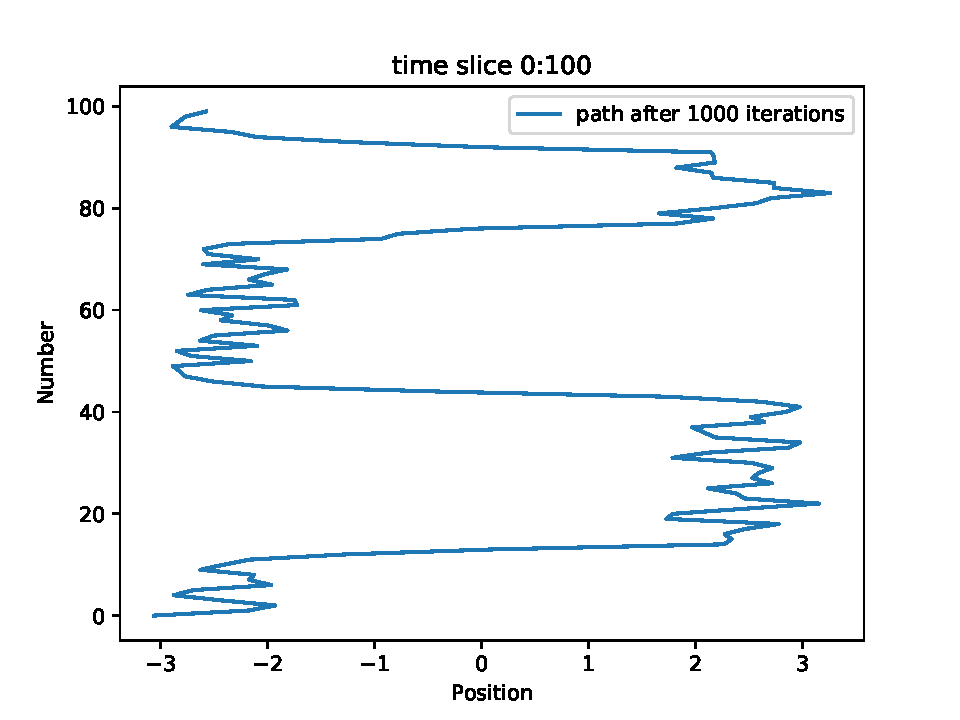
\includegraphics[width=\textwidth]{../imgs/anharmonic_oscillator_track/track_100010005_track_pretty_1000.pdf}
				\caption{Typical track of the anharmonic oscillator.}
				\label{fig:anharmonic_oscillator_track_100010005_track_pretty_1000}
			\end{figure}
		\end{column}
		\begin{column}{0.39\textwidth}
			\begin{itemize}
				\item Transitions between minima (at $\pm 2.5$) occur
				\\ $\Rightarrow$ Tunnelling effect
				\item Transitions are very fast, as expected
			\end{itemize}
		\end{column}
	\end{columns}
\end{frame}


\begin{frame}
	\frametitle{Measurements: linear energy-$\hbar$-dependence}
	\begin{figure}[H]
		\centering
			\begin{subfigure}[c]{0.45\textwidth}
				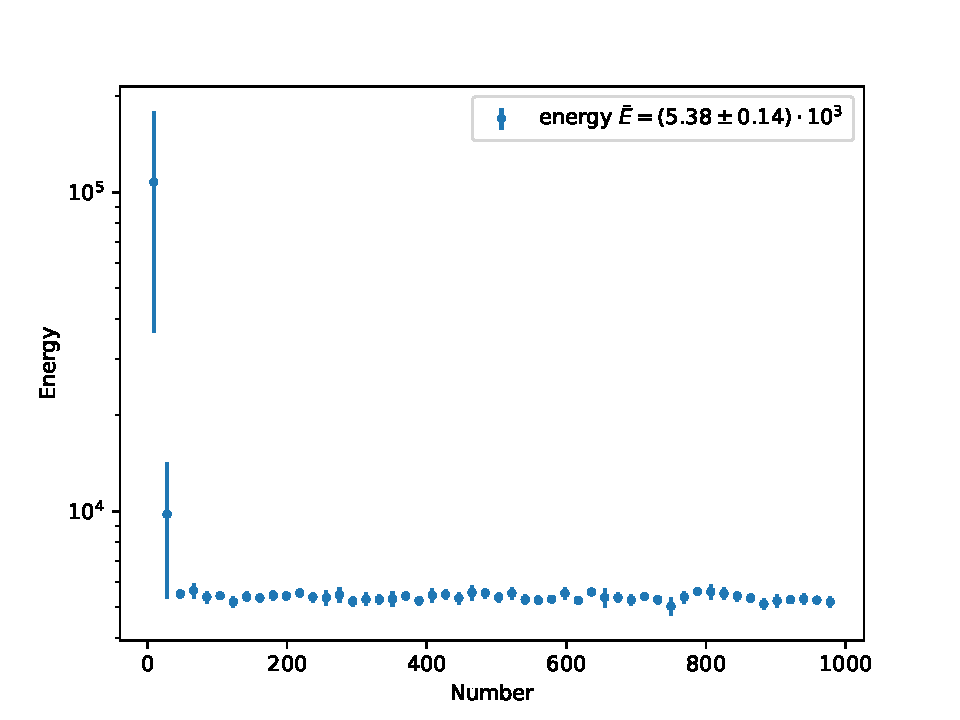
\includegraphics[width=\textwidth]{../imgs/harmonic_oscillator_track/track_10001000_thermalisation_log.pdf}
				\subcaption{Measurements}
			\end{subfigure}
			\begin{subfigure}[c]{0.45\textwidth}
				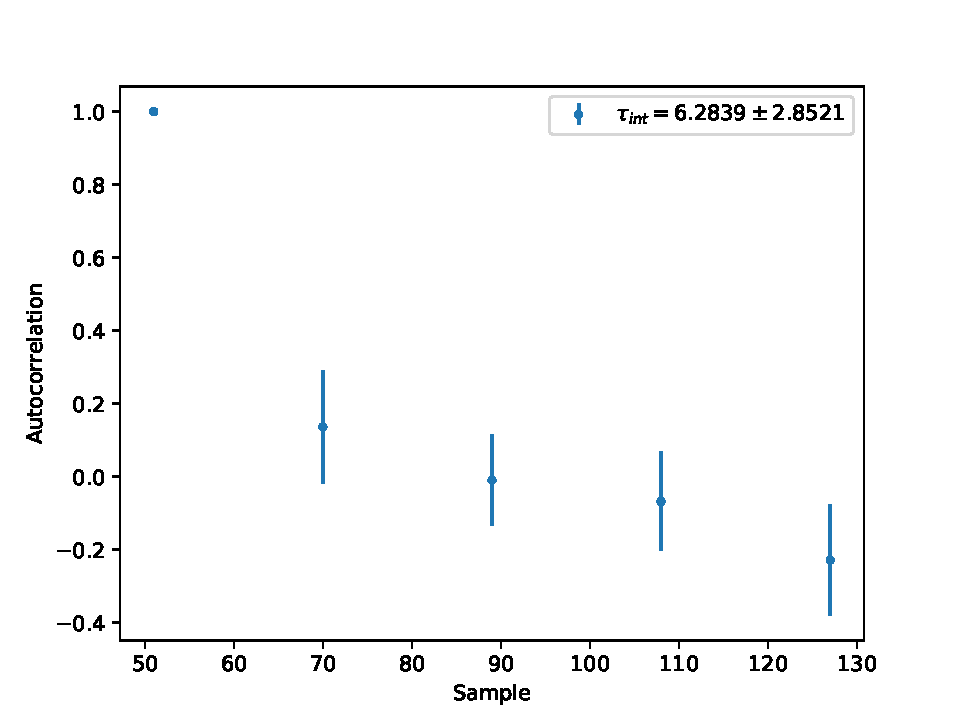
\includegraphics[width=\textwidth]{../imgs/harmonic_oscillator_track/track_10001000_thermalisation_log_autocorrelation.pdf}
				\subcaption{Autocorrelation}
			\end{subfigure}
		\label{fig:harmonic_oscillator_energy_measurement}
	\end{figure}
	\begin{itemize}
		\item Thermalisation of energy occurs after 50 iterations.
	\end{itemize}
\end{frame}


\begin{frame}
	\frametitle{Measurements: linear energy-$\hbar$-dependence}
	\vspace{-15px}
	\begin{columns}
		\begin{column}{0.6\textwidth}
			\begin{figure}[H]
				\centering
					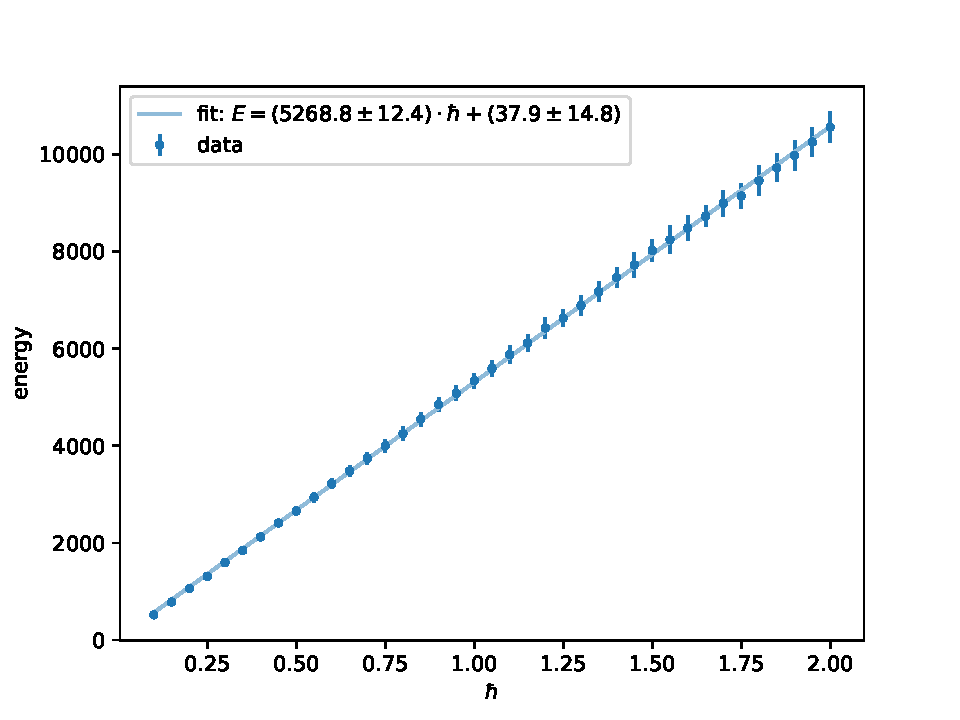
\includegraphics[width=\textwidth]{../imgs/harmonic_oscillator_classical_limit_energy/harmonic_oscillator_10_classical_limit_energy.pdf}
				\caption{Classical limit energy, harmonic oscillator.}
				\label{fig:harmonic_oscillator_classical_limit_energy}
			\end{figure}
		\end{column}
		\begin{column}{0.39\textwidth}
			\begin{itemize}
				\item Linear relation between $E$ and $\hbar$ as expected from $E = \hbar \omega \left(\frac 12 + n\right)$, for $n = 0$
				\item slope: $\frac\omega2=\SI{5268.8 +- 12.4}{}$
			\end{itemize}
		\end{column}
	\end{columns}
\end{frame}


\begin{frame}
	\frametitle{Measurements: tunnelling current}
	\vspace{-15px}
	\begin{columns}
		\begin{column}{0.6\textwidth}
			\begin{figure}[H]
				\centering
				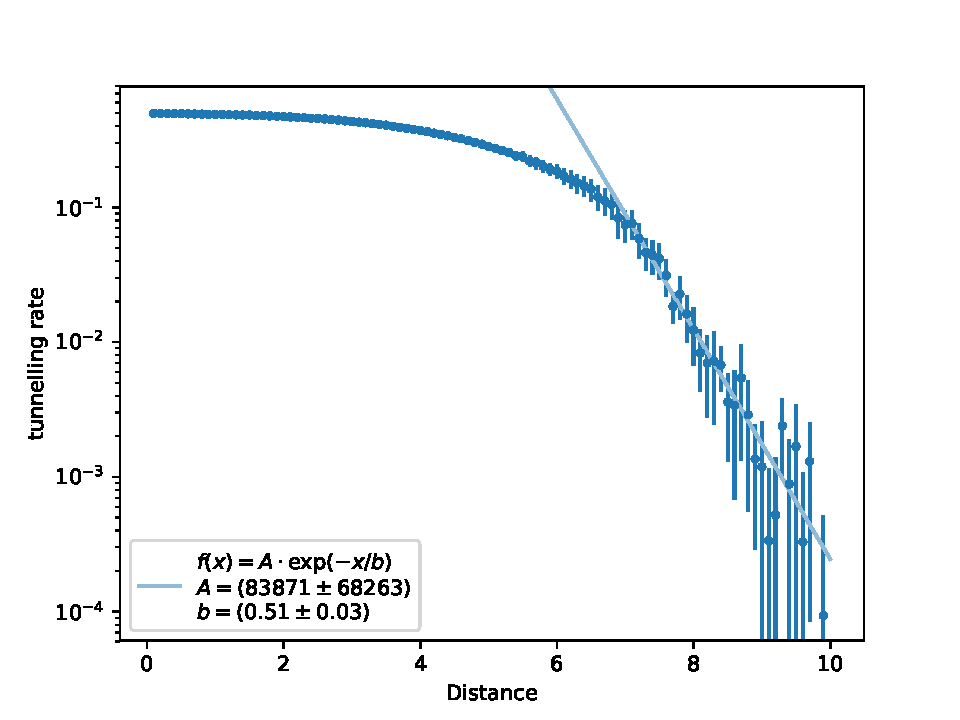
\includegraphics[width=\textwidth]{../imgs/anharmonic_oscillator_lambda_parameter/track_100001000_tunnelling_current_log_fit.pdf}
				\caption{Tunnelling current depending on the distance of the classical minima.}
				\label{fig:anharmonic_oscillator_tunnelling_current}
			\end{figure}
		\end{column}
		\begin{column}{0.39\textwidth}
			\begin{itemize}
				\item Behaviour is different for distances $d > 7$ and $d < 7$
				\item Tunnelling current decays exponentially with increased distance of minima for $d > 7$.
			\end{itemize}
		\end{column}
	\end{columns}
\end{frame}


\begin{frame}
	\frametitle{Measurements: Probability distribution}
	\vspace{-15px}
	\begin{columns}
		\begin{column}{0.55\textwidth}
			\begin{figure}[H]
				\centering
				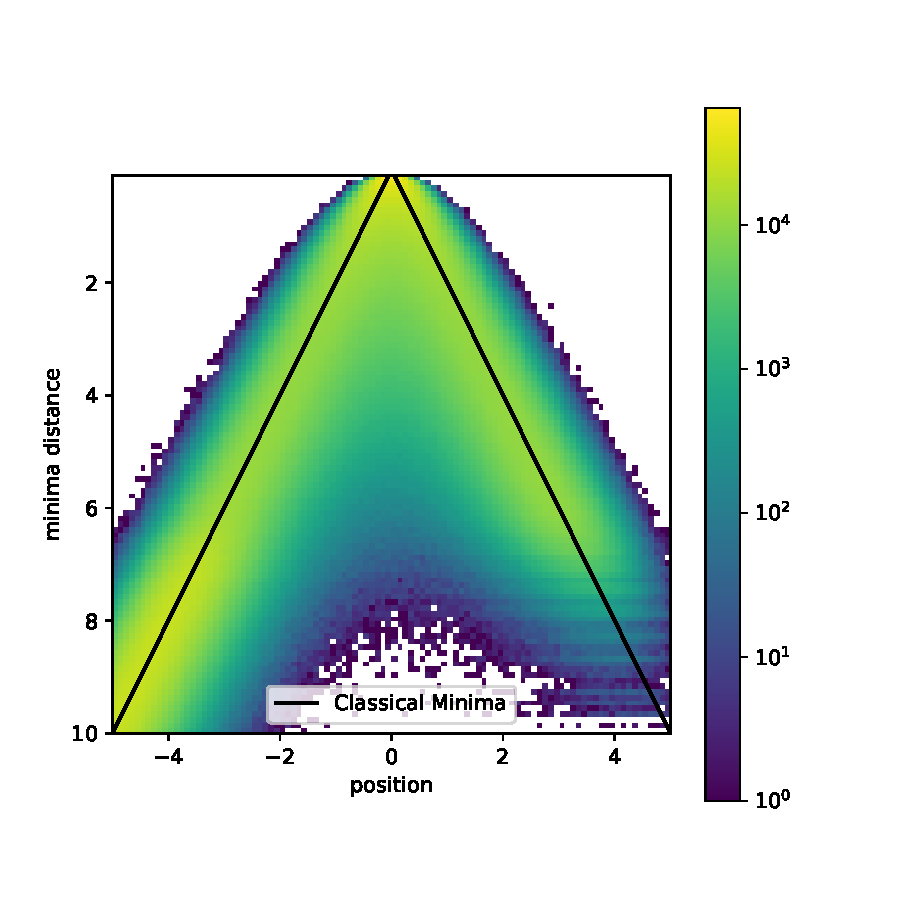
\includegraphics[width=\textwidth]{../imgs/anharmonic_oscillator_lambda_parameter/track_100001000_lambda_parameter.pdf}
				\label{fig:anharmonic_oscillator_lambda_parameter}
			\end{figure}
		\end{column}
		\begin{column}{0.44\textwidth}
			\begin{itemize}
				\item Initially prepared in the left minimum
				\item Distributions are centred around the classical limits
				\item Tunnelling occurs rarely for large distances of minima
			\end{itemize}
		\end{column}
	\end{columns}
\end{frame}


\begin{frame}
	\frametitle{Measurements: Virial theorem}
	\vspace{-10px}
	\begin{figure}[H]
		\centering
			\begin{subfigure}[c]{0.49\textwidth}
				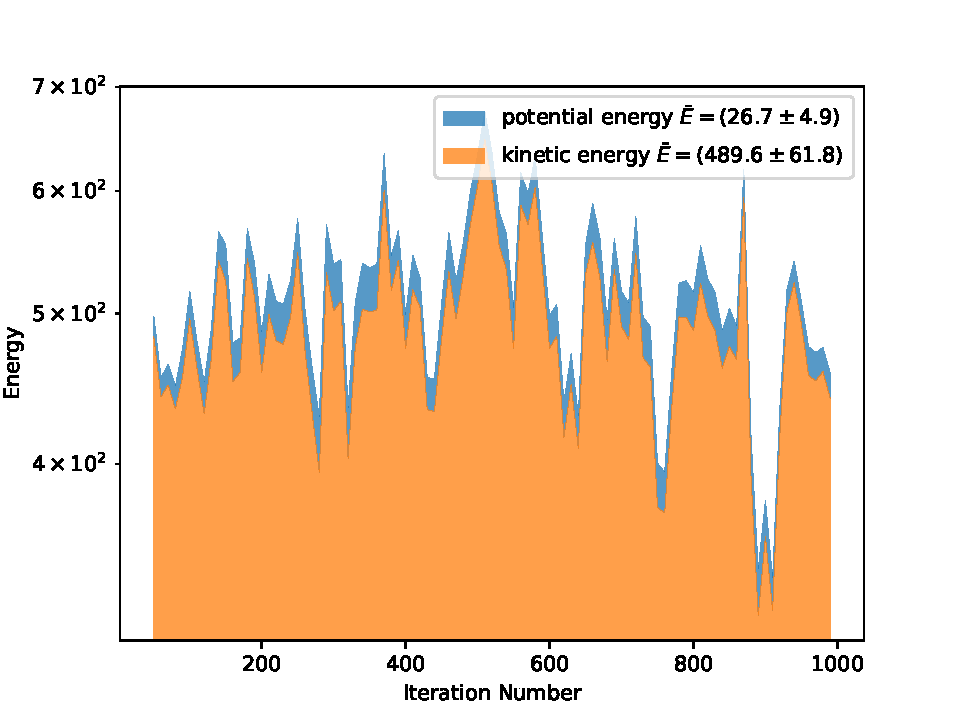
\includegraphics[width=\textwidth]{../imgs/harmonic_oscillator_track/track_1000100_heavy_virial_log.pdf}
				\subcaption{Using $m = 10$.}
				\label{fig:track_1000100_heavy_virial_log}
			\end{subfigure}
			\begin{subfigure}[c]{0.49\textwidth}
				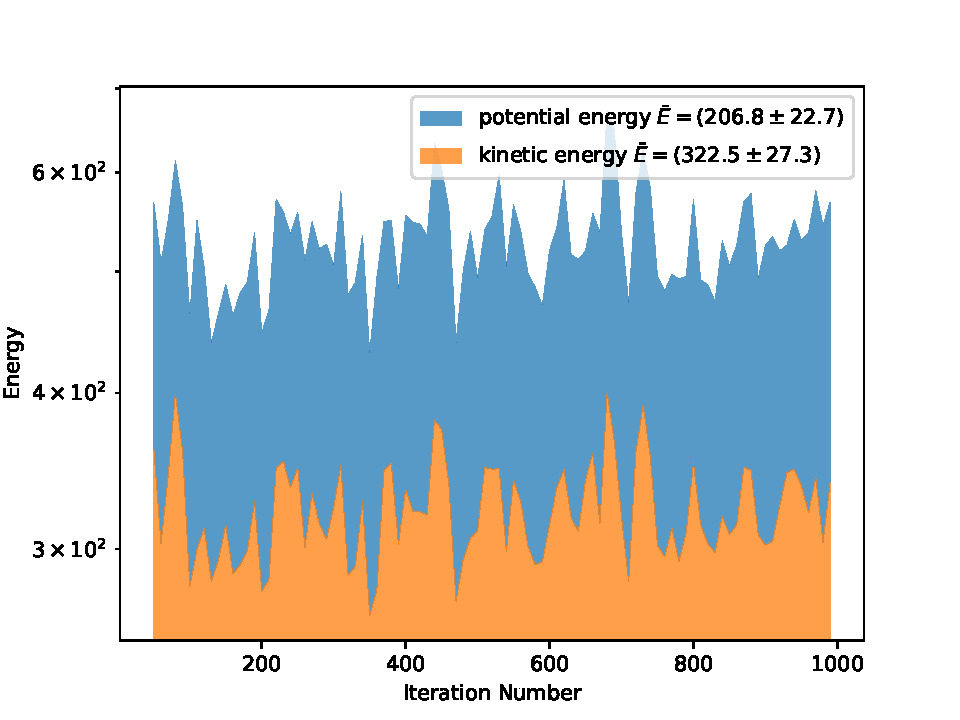
\includegraphics[width=\textwidth]{../imgs/harmonic_oscillator_track/track_1000100_virial_log.pdf}
				\subcaption{Using $m = 0.25$.}
				\label{fig:track_1000100_virial_log}
			\end{subfigure}
		%\caption{Distribution of the total energy into potential and kinetic part.}
		\label{fig:track_1000100_virial}
	\end{figure}
	\begin{itemize}
		\item Energy is not distributed evenly between kinetic and potential part
		\item Virial theorem does not hold for the produced data
	\end{itemize}
\end{frame}


\section{Summary}
\begin{frame}
	\frametitle{Summary}
	\begin{itemize}
		\item Classical limit confirmed validity of the code
		\item Metropolis-algorithm produces gaussian shaped distributions
		\item Linear relation between $E$ and $\hbar$ could be confirmed
		\item Tunnelling current could be measured depending on the difference of the minima
		\item The Virial theorem does not apply for the simulated data
	\end{itemize}
\end{frame}


\begin{frame}
\frametitle{}
\begin{center}
	Thank you for your attention!
\end{center}
\end{frame}

\section{References}
\begin{frame}
\setbeamertemplate{bibliography item}{\insertbiblabel}
\frametitle{References}
\newcounter{firstbib}
\vspace{-20px}
\begin{tiny}
	\begin{thebibliography}{99}
		\fontsize{6}{6}
		\bibitem{bender} C. M. Bender and T. T. Wu, \textit{Anharmonic oscillator}, Phys. Rev. (2) \textbf{184}, 1231–1260 (1969).
		\bibitem{rushka_freericks} M. Rushka J. K. Freericks, \textit{A Completely Algebraic Solution of the Simple Harmonic Oscillator}, arXiv:1912.08355 [quant-ph] (2019).
		\bibitem{creutz_freedman} M. Creutz and B. Freedman, \textit{A statistical approach to quantum mechanics}, Annals of Physics, \textbf{132}, 427-462 (1981).
		\bibitem{rodgers_raes} R. Rodgers and L. Raes, \textit{Monte Carlo simulations of harmonic and anharmonic oscillators in discrete Euclidean time}, DESY Summer Student Programme (2014).
		\bibitem{wick} G. C. Wick, \textit{Properties of Bethe-Salpeter Wave Functions}, Physical Review. \textbf{96} 1124–1134 (1954).
		\bibitem{carinena_falceto_ranada} J. F. Cari\~{n}ena, F. Falceto and M. F. Ra\~{n}ada, \textit{A geometric approach to a generalized virial theorem}, arXiv:1209.4584 [math-ph] (2012).
		\bibitem{github} Public Github repository: Harmonic Oscillator, Benedikt Otto (s6beotto), \\\url{https://github.com/s6beotto/Harmonic-Oscillator}.
		\bibitem{latexrun} Public Github repository: latexrun, Austin Clements (aclements), \\\url{https://github.com/aclements/latexrun}.
		\setcounter{firstbib}{\value{enumiv}}
	\end{thebibliography}
\end{tiny}
\end{frame}


\appendixstyle

\appendix

\section{Directory structure}
\subsection{Data generation}
\begin{frame}
\frametitle{Data generation}
	\begin{figure}[H]
		\centering
		\begin{tikzpicture}[scale=0.8, every node/.style={scale=0.8}]
			\draw[color=black, thick]
			node[draw,minimum width=2cm,minimum height=1cm,label=root,rounded corners=0.25cm] (root) at (0, 0){Harmonic-Oscillator}
			node[draw,minimum width=2cm,minimum height=1cm,rounded corners=0.25cm] (bin) at (-7.5, -2){bin/}
			node[draw,minimum width=2cm,minimum height=1cm,rounded corners=0.25cm] (bin_metropolis) at (-7.5, -4){libmetropolis.so}
			node[draw,minimum width=2cm,minimum height=1cm,rounded corners=0.25cm] (src) at (-2, -2){src/}
			node[draw,minimum width=2cm,minimum height=1cm,rounded corners=0.25cm] (src_create) at (-4, -4){(an)harmonic*.py}
			node[draw,minimum width=2cm,minimum height=1cm,rounded corners=0.25cm] (src_plot) at (0, -4){create\_plot*.py}
			node[draw,minimum width=2cm,minimum height=1cm,rounded corners=0.25cm] (data) at (2, -2){data/}
			node[draw,minimum width=2cm,minimum height=1cm,rounded corners=0.25cm] (imgs) at (6, -2){imgs/};
			\draw [->] (root) -- (bin);
				\draw [->] (bin) -- (bin_metropolis);
			\draw [->] (root) -- (src);
				\draw [->] (src) -- (src_create);
				\draw [->] (src) -- (src_plot);
			\draw [->] (root) -- (data);
			\draw [->] (root) -- (imgs);
			\draw [<->, thick, blue] (bin_metropolis) -- (src_create) node[midway,above=0.35] {C++ library};
			\draw [->, very thick, red] (src_create.east) -| ++(0.5, 1) -| (data) node[midway,below] {metropolis generation};
			\draw [->, very thick, red] (data) -- (imgs) node[midway,above] {plotting};
			\draw [->, thick, blue] (src_plot.east) -| (4, -2);
		\end{tikzpicture}
		\caption{Directory structure of the project for data generation.}
		\label{fig:scheme_dirs_data_generation}
	\end{figure}
\end{frame}


\subsection{Report generation}
\begin{frame}
\frametitle{Report generation}
	\begin{figure}[H]
		\centering
		\begin{tikzpicture}[scale=0.8]
			\draw[color=black, thick]
			node[draw,minimum width=2cm,minimum height=1cm,label=root,rounded corners=0.25cm] (root) at (0, 0){Harmonic-Oscillator}
			node[draw,minimum width=2cm,minimum height=1cm,rounded corners=0.25cm] (report) at   (-6,  -3){report/}
			node[draw,minimum width=2cm,minimum height=1cm,rounded corners=0.25cm] (imgs) at     (-2, -3){imgs/}
			node[draw,minimum width=2cm,minimum height=1cm,rounded corners=0.25cm] (latexrun) at (2,  -5){latexrun.py}
			node[draw,minimum width=2cm,minimum height=1cm,rounded corners=0.25cm] (build) at    (6,  -3){build/};
			\draw [->] (root) -- (report);
			\draw [->] (root) -- (imgs);
			\draw [->] (root) -- (latexrun);
			\draw [->] (root) -- (build);
			\draw [<-, thick, blue] (latexrun.west) + (0,-3mm) -| (report.south) node[midway,below] {*.tex};
			\draw [<-, thick, blue] (latexrun.west) + (0, 3mm) -| (imgs.south)   node[midway,below] {*.pdf};
			\draw [->, thick, blue] (latexrun) -| (build.south)                  node[midway,below] {report.pdf};
		\end{tikzpicture}
		\caption{Directory structure of the project for report generation.}
		\label{fig:scheme_dirs_report_generation}
	\end{figure}
\end{frame}


\end{document}
